\documentclass[a4paper,twoside]{article}

\usepackage{epsfig}
\usepackage{subcaption}
\usepackage{calc}
\usepackage{amssymb}
\usepackage{amstext}
\usepackage{amsmath}
\usepackage{amsthm}
\usepackage{multicol}
\usepackage{pslatex}
\usepackage{apalike}
\usepackage{tensor} 
\usepackage{cite}
\usepackage{floatrow}
\usepackage{blindtext}
%\usepackage{mathtools}
\usepackage{SCITEPRESS}     % Please add other packages that you may need BEFORE the SCITEPRESS.sty package.

\newtheorem{theorem}{Theorem}
\newtheorem{definition}{Definition}

\newcommand{\selfsim}{\mathop{\it selfsim}}
\newcommand{\dist}{\mathrm{dist}}
%\newcommand{\dim}{\mathrm{dim}}
\newcommand{\Ueps}{U_{\epsilon}}
\newcommand{\limeps}{\lim_{\epsilon \to 0}}
\newcommand{\delx}{\Delta x}
\newcommand{\Rone}{\mathbb{R}}
\newcommand{\Rtwo}{{\mathbb{R}}^2}
\newcommand{\Rn}{{\mathbb{R}}^n}
\newcommand{\Rm}{{\mathbb{R}}^m}
\newcommand{\Proj}{\mathrm{P}{\,}}
\newcommand{\Ima}{\mathrm{Im}{\,}}
\newcommand{\ProjNonOrth}[2]{\tensor*{\Proj}{^{#1}_{#2}}}
\newcommand{\Laplace}{\mathrm{\Delta}}
\newcommand{\LaplaceBeltrami}{\mathrm{\Delta_{{LB}}}}
%\newcommand{\partderiv}[2]{\frac{\partial #1}{\partial #2}}
\newcommand{\partderiv}[2]{\partial_{#2} {#1}}
\newcommand{\extr}[1]{\mathrm{extr}_{#1}}
\newcommand{\toreal}{\rightarrow\R}
\newcommand{\toeuclidean}[1]{\rightarrow\R^{#1}}
\newcommand{\CovariantDiffManif}[1]{\nabla^{#1}}
\newcommand{\CovariantDerivManif}[2]{\tensor*{\nabla}{^{#1}_{#2}}}
\newcommand{\CovariantDiff}{\nabla}
\newcommand{\CovariantDeriv}[1]{\nabla_{#1}}
\newcommand{\Diff}{\mathrm{d}}
\newcommand{\TangentSpaceArg}[2]{{T_{#2}}{#1}}
\newcommand{\CotangentSpaceArg}[2]{\tensor*{T}{^{*}_{#2}}{#1}}
\newcommand{\TangentBundle}[1]{T{#1}}
\newcommand{\CotangentBundle}[1]{\tensor*{T}{^{*}}{#1}}
\newcommand{\FRScalar}{BR_{\mathrm{scalar}}}
\newcommand{\FRMean}{BR_{\mathrm{mean}}}
\newcommand {\tr}{{\,}\mathrm{tr}{\,}}
\newcommand {\Preimage}[2]{{#2}^*{#1}}
\newcommand \TArgPreimage[3]{\Preimage{\TangentSpaceArg{#1}{#2}}{#3}}
\newcommand {\DiffSpaceArg}[4]{\CotangentSpaceArg{#1}{#2}\otimes \TArgPreimage{#2}{#3}}
\newcommand {\HessianSpaceP}[3]{\CotangentSpaceP{#1}\otimes \CotangentSpaceP{#1}\otimes \TpPreimage{#2}{#3}}

\newcommand \TPreimage[2]{\Preimage{\TangentBundle{#1}}{#2}}
\newcommand \CotPreimage[2]{\Preimage{\CotangentBundle{#1}}{#2}}
\newcommand \CotPPreimage[2]{\Preimage{\CotangentSpaceP{#1}}{#2}}
\newcommand {\DiffSpace}[3]{\CotangentBundle{#1}\otimes \TPreimage{#2}{#3}}
\newcommand {\HessianSpace}[2]{\CotangentBundle{#1}\otimes \CotangentBundle{#1}\otimes \TangentBundle{#2}}
\newcommand {\HessianSpaceF}[3]{\CotangentBundle{#1}\otimes \CotangentBundle{#1}\otimes \TPreimage{#2}{#3}}
\newcommand {\HessianSpaceFArg}[3]{\CotangentBundle{#1}\otimes \CotangentBundle{#1}\otimes \TPreimage{#2}{#3}}

\newcommand {\bigeps}{\mathcal{E}}

\begin{document}

\title{Corner Detection in Manifold-Valued Images and in Vector Fields }

\author{\authorname{Aleksei Shestov\sup{1}, Mikhail Kumskov\sup{1}}
\affiliation{\sup{1}Faculty of Mechanics and Mathematics, Lomonosov Moscow State University, 1 Leninskiye Gory, Moscow, Russia}
\email{\{shestov.msu,mkumskov\}@gmail.com}
}

\keywords{Corner Detection, Manifold-Valued Images, Vector Fields, Vector Bundles}

\abstract{This paper is devoted to the problem of corner detection in manifold-valued images and in vector fields on manifolds. Our solution is a generalization of the Harris corner detector \cite{Harris}. As in the grayscale case, our algorithm is based on an estimation of a self-similarity of a point neighborhood. We define the self-similarity for the general cases and obtain approximations of it by an action of a bilinear form. This form can be viewed as a generalization of the structure tensor \cite{StructureTensor}. The generalized structure tensor is then used as usual in the corner detection procedure. Finally, we describe future experiments: the algorithm will be tested on a task of chemical compounds classification.}

\onecolumn \maketitle \normalsize \setcounter{footnote}{0} \vfill

\section{\uppercase{Introduction}}
\label{sec:introduction}

\noindent In many applications and practical cases we process non-Euclidean data. Images with values on the circle (periodic data) are met in applications involving the phase of Fourier transform \cite{CircleData1, CircleData2}, interferometric synthetic aperture radar\cite{CircleData3}, or hue-component of an image. Spherical data appear when dealing with 3d directional information \cite{SphereData1, SphereData2} or with color images in chromaticity-brightness color space \cite{SphereData3}. SO(3)-valued data are processed in electron backscattered tomography \cite{SO3Data1, SO3Data2}. Images with values in the symmetric positive-definite matrices space are met in DT-MRI imaging \cite{SPDMatrixData1, SPDMatrixData2} or in processing covariance matrices associated to image pixels \cite{SPDMatrixData3}. 
\\
Manipulating tangent vector fields is a fundamental operation in areas such as dynamic systems, finite elements and geometry processing \cite{TangentProc}. Also, numerous applications in computer graphics require to manipulate tangent vector fields on surfaces, for example, texture synthesis, non-photorealistic rendering, computer-generated movies, animation \cite{VectorProc}.
\\
One approach to the manifold data processing is a generalization of grayscale image processing methods. Harris corner detector is a widely used method of keypoints detection in grayscale images. It has applications in image alignment, stitching, registration, 2d mosaics creation, 3d scene modeling and reconstruction, motion detection, object recognition, etc. The goal of the algorithm is to find points which neighborhoods are not self-similar in any direction, opposed to edges, which are self-similar in one direction, and to flat surfaces, which are self-similar in any direction. Self-similarity is assessed by the sum of squared differences between a region and a shifted region. This sum is approximated by an action of a bilinear form, called the structure tensor \cite{StructureTensor}. A corner response is calculated from the eigenvalues of the structure tensor, and corners are found as local maximums of the corner response.
\\
Our goal is to develop a generalization of the Harris corner detector for the general settings of a). an image being a map between manifolds and b). an image being a vector field on a manifold. The main question of the generalization is deriving the structure tensor. In order to derive it, we start from definitions of the self-similarity of a point neighborhood. These definitions are similar to the grayscale case, but have some modifications: in the manifold case we substitute the distances on the manifold for the differences, in the vector field case we use the parallel transport. Then we derive approximations of the self-similarity by the action of the bilinear form, which matrix consists of the image derivatives and the image metric. This bilinear form can be viewed as a generalization of the structure tensor. The generalized structure tensor is used as usual in the corner detection procedure.

\subsubsection*{Contributions:}
\begin{enumerate}
\item We are the first to provide the Harris corner detector generalization for the cases of an image being a map between manifolds and an image being a vector field on a manifold. 
\item We are the first to provide an interest point detector for the case of an image being a vector field on a manifold. 
\end{enumerate}

\section{\uppercase{The Harris corner detector overview}}

\noindent Let's start from a description of the Harris corner detector for the grayscale case. The setting of the problem is the following. Let $f:\Rn \to \Rone$ be a grayscale image. We want to find points which neighborhoods have a low self-similarity. The self-similarity is assessed by the sum of squared differences between a neighborhood and a shifted neighborhood:
$$\selfsim(\epsilon\delx) = \int_{U(x_0)} w(x) \big(f(x+\epsilon\delx) - f(x)\big)^2 dx,$$
where $\delx$ is a direction in which we estimate the self-semilarity, $\|\delx\| = 1$, $U(x_0)$ is a neighborhood of interest, $w(x)$ is a weight function, the Gaussian function is usually chosen as $w(x)$.
\\
Earlier corner detectors\cite{Moravec1980} tried to calculate this quantity directly. The direct calculation has such drawback that a number of directions $\delx$, in which we can calculate $\selfsim$, is limited. In the Harris corner detector this problem is solved by using an approximation of $\selfsim$ by the Taylor expansion. The expressions are the following:
$$f(x+\epsilon\delx) - f(x) = \epsilon\sum_i \frac{\partial f}{\partial x_i}(x)\delx_i + o(\epsilon);$$
\begin{multline*}
\big(f(x+\epsilon\delx) - f(x)\big)^2 = \epsilon^2\sum_{i, j}\frac{\partial f}{\partial x_i}\frac{\partial f}{\partial x_j}\delx_i\delx_j + \\
+ o(\epsilon^2) = \epsilon\delx\big(df_x^T df_x\big)\epsilon\delx^T + o(\Delta f^2)
\end{multline*}
\begin{multline*}\selfsim(\epsilon\delx) = \int_{U(x_0)} w(x) \big(f(x+\epsilon\delx) -\\
- f(x)\big)^2 dx = \epsilon\delx\Big(\int_{U(x_0)} w(x) \big(df_x^T df_x\big) dx\Big) \epsilon\delx^T + \\
+ o(\selfsim);\end{multline*}
So $\selfsim(\epsilon\delx)$ for small values of $\epsilon$ is approximated by the action of the bilinear form $S=\int_{U(x_0)} w(x) \big(df_x^T df_x\big) dx$. This bilinear form is called the structure tensor. 
\\
The whole corner detection algorithm is the following:
\begin{enumerate}
\item Calculate the structure tensor for ever pixel of an image
\item Calculate a corner response. In the article\cite{Tomasi91} it's suggested to use the direction-wise minimum of the self-similarity, which is estimated from the eigenvalues of $S$. In\cite{Harris} another response expression is used: $R=\det S - k (\tr S)^2$. A usage of this expression is computationally cheaper than a direct estimation of the eigenvalues of $S$, because it doesn't involve the square root calculation. 
\item Corners are found as local maximums of the chosen response, which have a high response value. 
\end{enumerate}
An example of the Harris corner detection result is presented in Fig. \ref{fig:example1}.

\begin{figure}[!h]
\setlength{\lineskip}{0pt}
\vspace{-3.0cm}
  \centering
   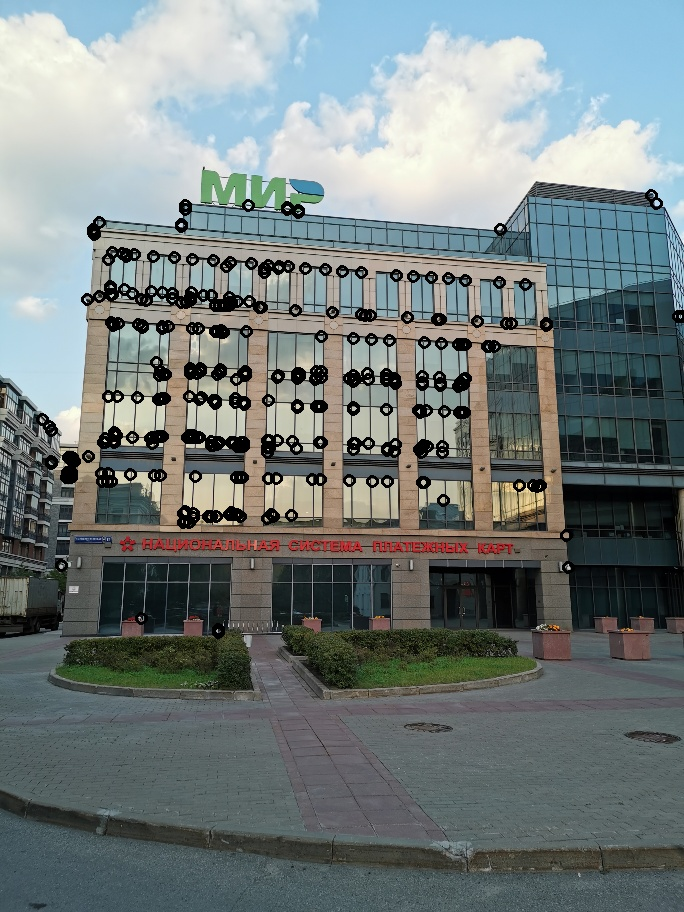
\includegraphics[scale=0.35,natwidth=684,natheight=912]{2.jpg} 
	%\hfill
	%\includegraphics[scale=0.25,natwidth=684,natheight=912]{3.jpg} 
  \caption{An image with found corners (denoted by black circles) on it.}
  \label{fig:example1}
 \end{figure} 

A generalization of the Harris corner detector for color images was proposed in the articles\cite{Montesinos98, Montesinos2000}. In these articles a norm of difference is used in $\selfsim$: 
$$\selfsim(\epsilon\delx) = \int_{U(x_0)} w(x) \|\big(f(x+\epsilon\delx) - f(x)\big)\|^2 dx.$$
This leads to the same expression for the matrix of the structure tensor, except now $df_x$ is a $3 \times n$ matrix.
\\
How can this algorithm be generalized to the more general data types? We can see that the real problem is the step 1 of the algorithm, the structure tensor calculation. So the main question is how to define the structure tensor. We will follow the next scheme:
\begin{enumerate}
\item We will define the self-similarity for the considered case. We can't straightforwardly use the self-similarity of the grayscale case, because some operations of it are not defined in the general case. So some modifications should be done to the self-similarity definition.
\item We will approximate the defined self-similarity for the small shifts by an action of a bilinear form, in order to be able to assess the self-similarity in every direction. This bilinear form will be used as the structure tensor in the corner detection algorithm.
\end{enumerate}

\section{\uppercase{The manifold case}}

\noindent Let us present our solution for the manifold case. In this case an image is a map between manifolds: $f(x): X \to Y$, where $X$ and $Y$ are Riemannian manifolds, $\dim(X) = n$, $\dim(Y) = m$. Here and further all manifolds and functions are considered to be smooth. A practical situation, corresponding to this general setting, could be, the following: $f$ is a chromaticity component of an image in the chromaticity-brightness color space\cite{SphereData3}. In the chromaticity-brightness model an RGB pixel value $I(x)$ is decomposed into 2 components --- the brightness component $u(x) = \|I(x)\|$, and the chromaticity component $f(x) = \frac{I(x)}{\|I(x)\|}$ (see Fig. \ref{fig:example2}). The chromaticity component $f(x)$ "lives" on a unit sphere $\mathbb{S}^2$. So for this case $X = A \subset \Rtwo$, $Y = \mathbb{S}^2$.

\begin{figure}[!ht]
\setlength{\lineskip}{0pt}
\vspace{-4.0cm}
  \centering
   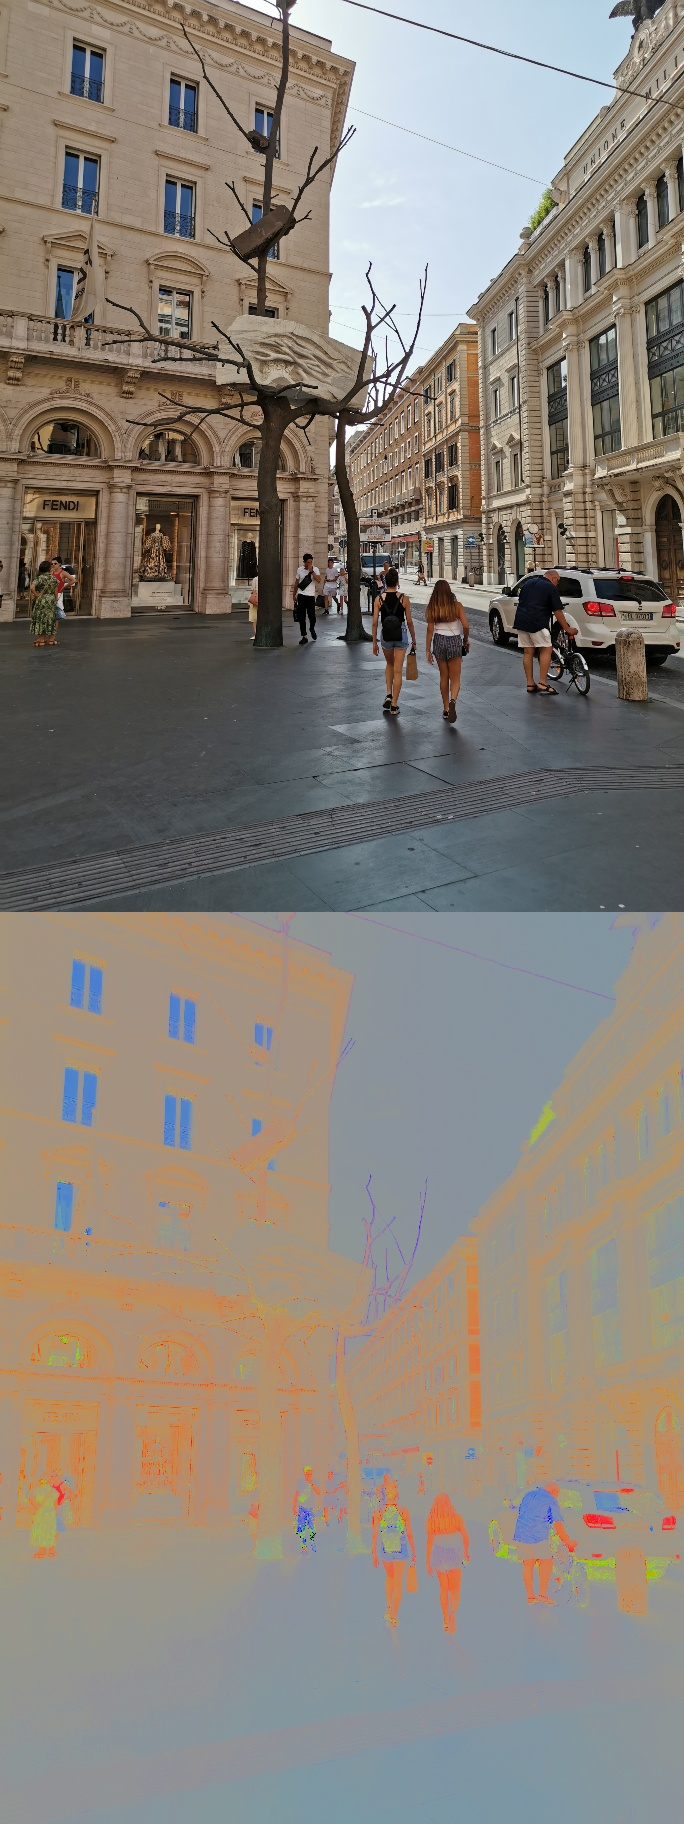
\includegraphics[scale=0.25,natwidth=684,natheight=1824]{6.jpg} 
  \caption{An image in the RGB space and its chromaticity component under it.}
  \label{fig:example2}
 \end{figure} 
At first, we should define the self-similarity for the considered case. As now $f(x)$ and $f(x + \epsilon\delx)$ are points on the manifold $Y$, we can't take the difference of them, because the difference is not defined in general. Instead we propose to take a length of the shortest path, connecting them on $Y$, as the distance. So self-similarity is defined in the following way (here $x+\epsilon\delx$ is a coordinate expression):
$$\selfsim(\epsilon\delx) = \int_{U(x_0)} w(x) \dist\big(f(x+\epsilon\delx), f(x)\big)^2 dx, $$
where $\|\delx\| = 1$. Then, as in the grayscale case, we will approximate the self-similarity for small shifts by the action of a bilinear form. This bilinear form can be viewed as a generalization of the structure tensor for the manifold case. The precise propositions are given in the following theorem. Before it we should state a few definitions.
\begin{definition}
Let $M$ be a smooth manifold, $\dim(M) = n$, $x \in M$. Pick a coordinate chart $\phi : U \to \Rn$, $x \in U$, $U \subset M$. Let there be two curves $\gamma_1, \gamma_2:(-1, 1) \to M$, $\gamma_1(0) = \gamma_2(0) = x$. $\gamma_1$ and $\gamma_2$ are equivalent at $x$ if and only if the derivatives of $\phi \circ \gamma_1$ and $\phi \circ \gamma_2$ at 0 coincide. Equivalence classes, defined in that way, are \textit{tangent vectors} of $M$ at $x$. Then the \textit{tangent} space of $M$ at $x$, denoted by $T_x M$, is a set of all tangent vectors of $M$ at $x$. $T_x M$ forms a linear space of $\dim(T_x M) = n$.
\end{definition}

\begin{definition}
Let $M$ be a smooth manifold, $\dim(M) = n$, $x \in M$. A metric tensor of $M$ at $x$ is a symmetric positive-definite bilinear form $g_x^M$, which acts on vectors of the tangent space $T_x M$. The length of a vector $v \in T_x M$ is defined as $\sqrt{g_x^M(v, v)}$.
\end{definition}

\begin{theorem}\label{ManifoldCase}
\begin{multline*}\selfsim(\epsilon\delx) = \\
=\epsilon\delx\Big(\int_{U(x_0)} w(x) \big(df_x^T G^Y_{f(x)} df_x\big) dx\Big) \epsilon\delx^T +\\
+ o(\selfsim),\end{multline*}
where $df_x$ is an $m \times n$ matrix of the differential of $f$ at the point $x$,
\\
$G^Y_{f(x)}$ is an $m \times m$ matrix of the metric of $Y$ at the point $f(x)$.
\\
The matrix $\int_{U(x_0)} w(x) \big(df_x^T G^Y_{f(x)} df_x\big) dx$ is the manifold structure tensor.
\end{theorem}
\begin{proof}
At first, let's approximate the distance between $f(x)$ and $f(x + \epsilon\delx)$ by their per-coordinate difference. Let $\gamma(t)$ be the shortest curve  in the natural parametrization connecting them: $\gamma(0) = f(x), \gamma(s) = f(x + \epsilon\delx), s=\dist(f(x), f(x + \epsilon\delx))$. Then by the Taylor expansion of $\gamma$:
$$f(x + \epsilon\delx) - f(x) = \dot{\gamma}(0) s + o(s).$$
Here $f(x + \epsilon\delx) - f(x) = \Delta f$ is a coordinate expression, $\dot{\gamma}(0)$ is a vector in the coordinates of $T_{f(x)}Y$,  $\dot{\gamma}(0)$ has a unit length. From this it also follows that $\Delta f = O(s)$. Then substitute this expression for the squared length of $\dot{\gamma}(0) s$:
$$s^2 g_y^Y (\dot{\gamma}(0), \dot{\gamma}(0)) = g_y^Y(\Delta f, \Delta f) + o(s^2), $$
where $g_y^Y$ is a metric tensor of $Y$ at the point $y=f(x)$.
$$\dist(f(x), f(x + \epsilon\delx))^2 = g_y^Y(\Delta f, \Delta f) + o(dist^2). $$
Let's approximate $\Delta f$ by the Taylor expansion: $\Delta f = df_x(\epsilon\delx) + o(\epsilon).$ Then
$$g_y^Y(\Delta f, \Delta f) = g_y^Y(df_x(\epsilon\delx), df_x(\epsilon\delx)) + o(\epsilon^2).$$
From the Taylor expansions: $\epsilon = O(\Delta f) = O(dist)$. Then 
\begin{multline*} \dist(f(x), f(x + \epsilon\delx))^2 = \\
= g_y^Y(df_x(\epsilon\delx), df_x(\epsilon\delx)) + o(dist^2) = \\
= \epsilon\delx\Big(\big(df_x^T G^Y_{f(x)} df_x\big) dx\Big) \epsilon\delx^T + o(dist^2).
\end{multline*}
Then 
\begin{multline*} 
\selfsim(\epsilon\delx) = \\
= \int_{U(x_0)} w(x) \dist\big(f(x+\epsilon\delx), f(x)\big)^2 dx = \\
=\epsilon\delx\Big(\int_{U(x_0)} w(x) \big(df_x^T G^Y_{f(x)} df_x\big) dx\Big) \epsilon\delx^T + \\
+ o(\selfsim)
\end{multline*}
\end{proof}

So we approximated the self-similarity by the action of the bilinear form $S = \int_{U(x_0)} w(x) \big(df_x^T G^Y_{f(x)} df_x\big) dx$. This bilinear form will be called the manifold structure tensor. It is then used as usual in the corner detection procedure: we calculate the corner response as the minimal eigenvalue of $S$, or calculate $R=\det S - k (\tr S)^2$. Corners are found as local maximums of the chosen response, which have high response values.
\section{\uppercase{The vector field case}}
\noindent Let us proceed to the case of image being a vector field on a manifold. Before going into more detailed discussion we need to state a few definitions.
\\
At first, let us discuss the notion of the vector bundle. Informally, the idea is the following: to every point $x$ of the manifold $X$ we attach a vector space $V(x)$ in such a way that these vector spaces fit together to form another manifold $E$, which is then called a vector bundle over $X$. I.e. vector bundles are spaces, where vector fields on a manifold "live". The formal definition is the following: 
\begin{definition}
A vector bundle $(E, X, \pi)$ consists of manifolds $X$ (base space), $E$ (total space) and a continuous surjection $\pi : E \to X$ (bundle projection). For every $x \in X$ $\pi^{-1}(x)$ (called a fiber) has the structure of a finite-dimensional vector space. The following condition is satisfied: for every point $x \in X$, there is an open neighborhood $U \subset X$ of $x$, and a homeomorphism

$$\phi : U\times \Rm \to \pi ^{-1}(U)$$
such that for all $x \in U$,
\begin{enumerate}
\item $(\pi \circ \phi )(x,v)=x$ for all $v \in \Rm$, 
\item the map $v\mapsto \phi (x,v)$ is a linear isomorphism between the vector spaces $\Rm$ and $\pi^{-1}(x)$. 
\end{enumerate}
\end{definition}
Elements of a vector bundle are called sections of a vector bundle. A section of a vector bundle can be simply viewed as a vector field on a manifold. The tangent bundle is also a vector bundle. 
\\
Proceed to the notion of the covariant derivative. The covariant derivative is a rule of calculating a derivative of sections of vector bundles. The formal definition is the following:
\begin{definition}
A covariant derivative $\nabla$  at a point $x$ in a smooth manifold $X$  assigns a section $(\nabla_v u)_x$ to a pair of a tangent vector $v$ at $x$ and a vector field $u$ defined in a neighborhood of $x$, such that the following properties hold:
\begin{enumerate}
\item $\nabla_v u$ is linear in $v$:
$$\nabla_{g v_1 + f v_2} u = g\nabla_{v_1} u + f\nabla_{v_2} u;$$
\item $\nabla_v u$  is additive in $u$:
$$\nabla_{v} u_1 + u_2 = \nabla_{v} u_1 + \nabla_{v} u_2;$$
\item $\nabla_v u$ obeys the product rule:
$$\nabla_v f u = f(x) \nabla_v u + u(x)\nabla_v f$$
\end{enumerate}
\end{definition} 
Now let us review the notion of the parallel transport. Informally speaking, the parallel transport is a way of transporting vectors from different fibers of a vector bundle along smooth curves in a manifold, so that they stay parallel with respect to the covariant derivative. The formal definition is the following:
\begin{definition}
Let $(E, X, \pi)$ be a vector bundle over $X$, let $e \in E_x$ at $x = \gamma(0) \in X$. The parallel transport of $e$ along $\gamma$ is the extension of $e$ to the unique section $u$ of $E$ along $\gamma$ such that:
\begin{enumerate}
\item $\nabla_{\dot{\gamma}} u = 0$;
\item $u_{\gamma (0)}=e$.
\end{enumerate}
\end{definition}
Then return to our problem. Let there be a manifold $X$, $\mathrm{dim}(X) = n$, a vector bundle $(E, X, \pi)$ over $X$, $\mathrm{dim}(E) = m$, and let $f$ be a section of this vector bundle ($f$ is a vector field on $X$). A particular case, corresponding to this general setting, could be, for example, the following: $X$ is a 2d surface and $f$ is a tangent vector field on $X$.
\\
At first, we should define the self-similarity for the considered case. In this case $f(x)$ and $f(x + \epsilon\delx)$ are elements of different fibers, so we can't take a difference of them. In order to manipulate them, these vectors should be moved by the parallel transport to the same fiber. So the self-similarity is defined in the following way (here $x+\epsilon\delx$ is a coordinate expression): 
\begin{multline*}\selfsim(\epsilon\delx) = \\
= \int_{U(x_0)} w(x) \|f(x+\epsilon\delx) - \Gamma_x^{x+\epsilon\delx}(f(x))\|^2 dx,
\end{multline*}
where $\|\delx\| = 1$, $\Gamma_x^{x+\epsilon\delx}$ denotes the parallel transport from $x$ to $x+\epsilon\delx$ along the shortest curve, connecting $x$ and $x+\epsilon\delx$. We assume that all operations take place in the normal neighborhood of $x$, that is a neighborhood, in which there is only one shortest curve, connecting each pair of points. Then, as in all previous cases, we will approximate the self-similarity for small shifts by the action of a bilinear form, which can be viewed as a generalization of the structure tensor to the vector field case. The formal expressions are given by the following theorem:
\begin{theorem}
\label{VectorFieldCase}
\begin{multline*}\selfsim(\epsilon\delx) = \\
=\epsilon\delx\Big(\int_{U(x_0)} w(x) \big(\nabla f_x^T G^E_{x} \nabla f_x\big) dx\Big) \epsilon\delx^T + \\
+ o(\selfsim),\end{multline*}
where $\nabla f_x$ is an $m \times n$ matrix of the covariant differential of $f$ at the point $x$, i.e. a matrix consisting of covariant derivatives of $f$ by the basis vectors: $\nabla f_x (i, j) = (\nabla_{e_j} f) (i)$
\\
$G^E_x$ is an $m \times m$ matrix of the metric of $E$ at the point $x$.
\\
The matrix $\int_{U(x_0)} w(x) \big(\nabla f_x^T G^E_{x} \nabla f_x\big) dx$ is the vector field structure tensor.
\end{theorem}
\begin{proof}
At first let's review the difference of the vectors:
\begin{multline*} f(x+\epsilon\delx) - \Gamma_x^{x+\epsilon\delx}(f(x)) = \\
= \frac{\epsilon (f(x+\epsilon\delx) - \Gamma_x^{x+\epsilon\delx}(f(x)))}{\epsilon} = \\
= \textrm{(by one of the properties) }\epsilon(\nabla_{\delx} f)_{x+\epsilon\delx} + o(\epsilon).
\end{multline*}
Let $x_1 = x+\epsilon\delx$. Then substitute this to the squared norm:
\begin{multline*} 
 \|\epsilon(\nabla_{\delx} f)_{x_1} + o(\epsilon)\|^2 = \\
= g^E_{x_1}(\epsilon(\nabla_{\delx} f)_{x_1}, \epsilon(\nabla_{\delx} f)_{x_1}) + o(\epsilon^2) = \\
= (g^E_{x} + o(\epsilon))(\epsilon(\nabla_{\delx} f)_{x} + o(\epsilon), \epsilon(\nabla_{\delx} f)_{x} + o(\epsilon)) + \\ 
+ o(\epsilon^2) = \epsilon\delx\big(\nabla f_x^T G^E_{x} \nabla f_x\big) \epsilon\delx^T + o(\epsilon^2).
\end{multline*}
From the Taylor expansion of $f$ $o(\epsilon^2) = o(\Delta f^2)$. Combine this with the self-similarity definition and obtain:
\begin{multline*}\selfsim(\epsilon\delx) = \\
= \int_{U(x_0)} w(x) \|f(x+\epsilon\delx) - \Gamma_x^{x+\epsilon\delx}(f(x))\|^2 dx = \\
= \epsilon\delx\Big(\int_{U(x_0)} w(x) \big(\nabla f_x^T G^E_{x} \nabla f_x\big) dx\Big) \epsilon\delx^T + \\
+ o(\selfsim).
\end{multline*}
\end{proof}
With this theorem we approximated the self-similarity by the action of the bilinear form $S = \int_{U(x_0)} w(x) \big(\nabla f_x^T G^E_{x} \nabla f_x\big) dx$. This bilinear form will be called the vector field structure tensor. It is then used as usual in the corner detection procedure: we calculate the corner response as the minimal eigenvalue of $S$, or calculate $R=\det S - k (\tr S)^2$. Corners are found as local maximums of the chosen response, which have high response values.

\section{\uppercase{The experiments}}
Regarding the experiments our work now is a work in progress. Here we will describe the future experimental setup and the algorithm implementation. These experiments were not conducted yet.
\subsection{Experimental Setup}
We will apply our blob detection framework to a chemical compounds classification problem, also called the QSAR problem \cite{qsar}. The task is to predict the activity of the compounds using their structure. Each compound is represented by a triangulated molecular surface \cite{molecular} and several physico-chemical and geometrical properties on the surface. We use the following properties: the electrostatic and the steric potentials, the Gaussian and the mean curvatures, the directions of electrostatic and steric forces, the gradients of the scalar properties. These properties are calculated in each triangulation vertex. So an input data element can be modeled as a 2-dimensional manifold $X$ with a combined function $(f_1, f_2, f_3)$: $f_1(x):X \to \Rone^4$ (the scalar properties), $f_2(x):X \to \mathbb{S}^2\times\mathbb{S}^2$ (the directional properties), $f_3$ is a section of the vector bundle $TX \otimes TX \otimes TX \otimes TX$ (the gradient properties). An example of input data is presented in Fig. \ref{fig:example3}

\begin{figure}[!h]
\setlength{\lineskip}{0pt}
\vspace{-1.5cm}
  \centering
   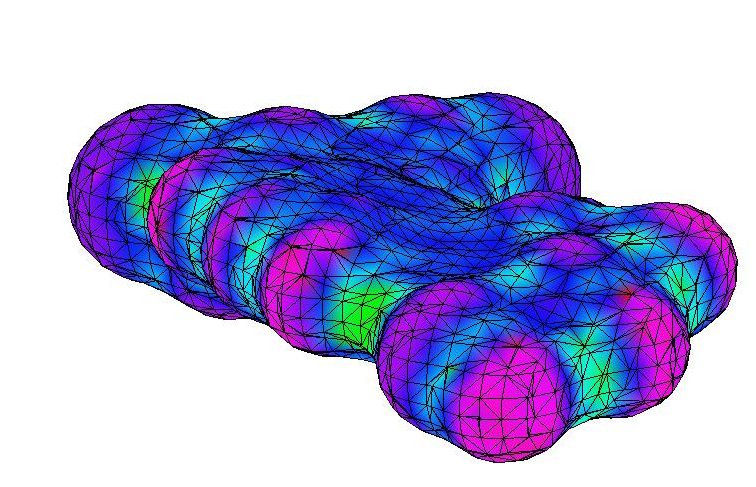
\includegraphics[scale=0.35,natwidth=756,natheight=487]{7.png} 
	%\hfill
	%\includegraphics[scale=0.25,natwidth=684,natheight=912]{3.jpg} 
  \caption{A molecular surface of a glycoside compound with the Gaussian curvature on it, denoted by color. Green is for low values, red is for high values.}
  \label{fig:example3}
 \end{figure} 

\subsection{Implementation}
We use the manifold and vector field corner detectors for the construction of descriptor vectors. The procedure is the following:
\begin{enumerate} 
\item Detect corners by our method on each compound surface;
\item	Form pairs of corners on each surface;
\item Transform the corners pairs into vectors of the same length by using the bag of words approach \cite{bag}.
\end{enumerate}
The implementation of the procedure of the corner detection is the following:
\begin{enumerate} 
\item Calculate the differentials of each component of $f_1$ and $f_2$ by the approach following\cite{GradLeastSQR}. The differentials of $f_2$ are calculated for each coordinate $\phi$ and $\theta$ of the spherical coordinate system. The overall differentials $df_1$ and $df_2$ are obtained by stacking per-component differentials: $df_1 = (df_{11}, df_{12}, df_{13}, df_{14})$, $df_2 = (df_{21\phi}, df_{21\theta}, df_{22\phi}, df_{22\theta})$. The procedure of the differentials $df_{ik}$ calculation is the following:
\begin{itemize}
			\item Find the directional derivatives $\partderiv{f_{ik}}{z_j}$ by the finite differences approximation, where $z_j$̅ are the directions from $v$ to its neighbour vertices. 
			\item Find the differential $\Diff f_i=(\Diff f_{ik})$ by solving the overdetermined linear system $\Diff f(Z)=\partderiv{f_{ik}}{z_j}$ , $Z$  is a matrix which columns are vectors $z_j$.
\end{itemize}
\item Calculate the covariant differentials $\nabla f_{3k}$ of each component of $f_3$ by the approach following\cite{CovariantCalc}. The overall covariant differential $\nabla f_3$ is obtained by stacking per-component covariant differentials $\nabla f_3 = (\nabla f_{31}, \nabla f_{32}, \nabla f_{33}, \nabla f_{34})$
\item Calculate matrices under the integral of the structure tensor definition
\begin{itemize}
		\item Calculate $S_{01}=df_1^T G^{\Rone^4}_{f_1(x)} df_1$ (see the Theorem \ref{ManifoldCase}) for $f_1$. For the $f_1$ case the matrix  $G^{\Rone^4}_{f_1(x)}$ is simply a unit matrix.
		\item Calculate $S_{02}=df_2^T G^{\mathbb{S}^2\times\mathbb{S}^2}_{f_2(x)} df_2$ (see the Theorem \ref{ManifoldCase}) for $f_2$. For the $f_2$ case the matrix $G^{\mathbb{S}^2\times\mathbb{S}^2}_{f_2(x)}$ is found by the standard formulas for the spherical coordinate system.
		\item Calculate $S_{03}=\nabla f_3^T G^{TX^4}_{x} \nabla f_3$ (see the Theorem \ref{VectorFieldCase}) for $f3$. For the $f_3$ case the matrix  $G^{TX^4}_{x}$ is simply a unit matrix, because we chose an orthonormal coordinate system at each vertex.
		\item Calculate $S_{0} = S_{01} + S_{02} + S_{03}$.
\end{itemize}
\item For each vertex calculate the structure tensor $S(x_0) = \int_{U(x_0)} w(x) S_{0} dx$ with different values of $w(x)$. We choose the Gaussian function with different values of $\sigma$ as $w(x)$.
\item Detect corners as local maximums of the corner response $R=\det S - k (\tr S)^2$ for each value of $\sigma$ of $w(x)$.
\end{enumerate}

\section{\uppercase{Conclusion}}
We propose the framework for the corner detection in manifold-valued images and in vector fields over manifolds. This framework is based on the approximation of the self-similarity by the action of the structure tensor. Both the self-similarity and the structure tensor are derived in our work for the general cases. Our approach gives new methods for the uncovered problems. The future experiments and the implementation are described. The next direction for the research is the described experiment.

\bibliographystyle{apalike}
{\small
\bibliography{article_3}}

\end{document}

